\documentclass[tikz]{standalone}
\usepackage{ctex}
\usepackage{tikz}
\usepackage{pgfplots}
\pgfplotsset{compat=1.18}   % 使用较新版本语法
\usetikzlibrary{positioning, arrows.meta, intersections, calc, fit, backgrounds}
\usepgfplotslibrary{fillbetween}  % 用于填充区域

\begin{document}
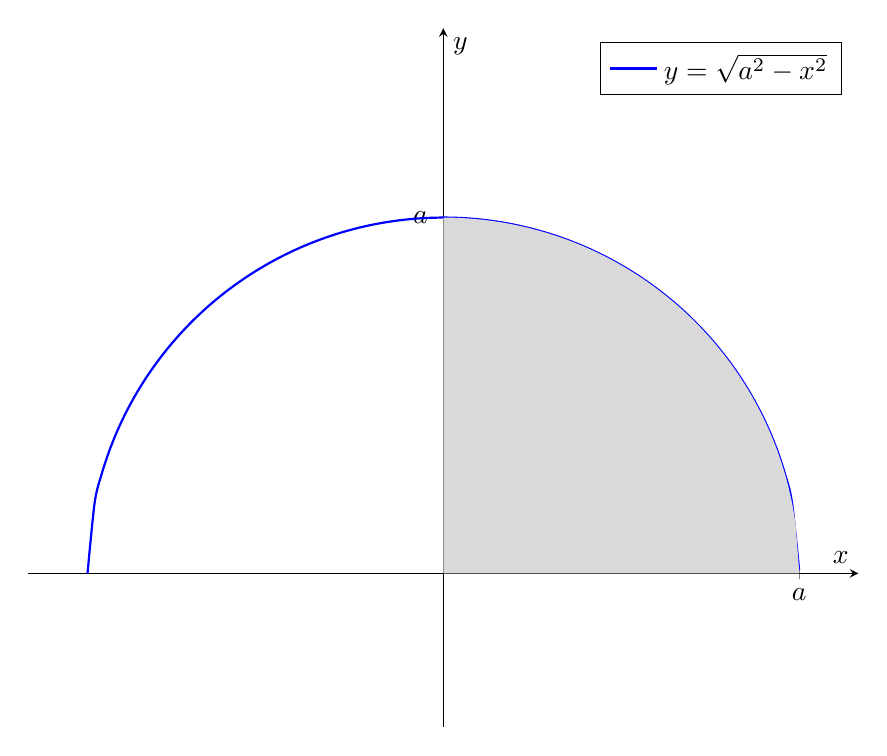
\begin{tikzpicture}
    % 定义参数 a
    \pgfmathsetmacro{\a}{3}

    \begin{axis}[
            axis lines = middle,          % 坐标轴穿过原点
            xlabel = $x$, ylabel = $y$,
            xmin = -\a-0.5, xmax = \a+0.5,
            ymin = -0.2, ymax = \a+0.5,
            xtick = {0, \a},              % 只显示 0 和 a 的刻度
            xticklabels = {0, $a$},
            ytick = {\a},
            yticklabels = {$a$},
            samples = 100,                % 提高曲线平滑度
            axis equal = true,            % 保持横纵比例一致（显示真实的圆）
            clip = false,                 % 允许标注超出轴范围
            every axis plot post/.append style={thick},
            width=\textwidth
        ]

        \addplot[domain=-\a:\a, smooth, thick, blue]
        {sqrt(\a^2 - x^2)};
        \addlegendentry{$y=\sqrt{a^2-x^2}$}

        % 2. 填充从 0 到 a 的积分区域（曲线与 x 轴之间）
        \addplot[fill=gray!30, draw=none, domain=0:\a]
        {sqrt(\a^2 - x^2)} \closedcycle;
    \end{axis}
\end{tikzpicture}
\end{document}